\documentclass{article}

\usepackage[nonatbib, preprint]{neurips_2019}
 
\usepackage[utf8]{inputenc} % allow utf-8 input
\usepackage[T1]{fontenc}    % use 8-bit T1 fonts
\usepackage{hyperref}       % hyperlinks
\usepackage{url}            % simple URL typesetting
\usepackage{booktabs}       % professional-quality tables
\usepackage{amsfonts}       % blackboard math symbols
\usepackage{nicefrac}       % compact symbols for 1/2, etc.
\usepackage{microtype}      % microtypography
\usepackage{graphicx}
\usepackage{amsmath}

\title{Applying Dimensionality Reduction and Deep Learning to Network Intrusion Detection}

\author{
  Brant Geddes\\
  Faculty of Engineering and Applied Science, University of Regina, SK, Canada S4S 0A2\\
  geddes2b@uregina.ca
}

\begin{document}

\maketitle

\begin{abstract}
  With network threats evolving quickly, it is crucial for administrators to react in kind and deploy smarter solutions. One area that is quickly evolving is Network Intrusion Detection, where a service can be trained to classify threats as they happen and take the appropriate actions. Due to how quickly new threats evolve, machine learning algorithms are best suited to classifying threats due to the ability to train them on newly acquired data without needing a subject matter expert to define rules for the system. This paper presents a stacked encoder architecture for dimensionality reduction that feeds into a dense neural network used to classify the data based on the reduced feature set. The proposed model was trained using the Tensorflow library and evaluated on the NSL-KDD dataset. Oversampling was used to compensate for the imbalance in label numbers and help improve the accuracy of classes with low representation in the set. The model shows positive results, with a low training time and high accuracy which will only become stronger as more data in this field is acquired.
\end{abstract}

\section{Introduction}

An important topic in the area of networking and computing is network security. Network security can be broken into two main areas of practice, proactive and reactive. Proactive security practices are steps taken to mitigate threats before they happen. This can encompasses everything from encryption protocols, network design, server configuration, and best practices for users. Reactive security practices are steps taken to discover a threat that has happened and mitigate damages. This can take the form of monitoring access logs, intrusion detection systems, data anonymization, and data backups. It is important to provide a certain level of proactive security in order to safeguard against unauthorized access to the network, but this cannot be relied on due to how quickly threats evolve. It is inevitable that an adversary bypasses security and gains access to the system. Due to this, a level of reactive security is important to both show the existence of an attack and to allow administrators to take the necessary steps to reduce to amount of damage done by the attack. One form of reactive security is known as Network Intrusion Detection (NID). 
\\
A NID is software that monitors various network parameters and attempts to classify interactions as normal or malicious. These systems cannot stop an adversary from gaining access to the system, but it can identify malicious activity quickly and take appropriate action. There are several ways to implement a NID, such as an expert system or a supervised machine learning model. An expert system is built by a subject matter expert who manually programs rules the system should follow. This method requires an expert in network security with knowledge of existing threats to spend time manually teaching an artificial intelligence how to identify malicious activity. Expert systems are viable when the subject matter is static or changes slowly, which is not the case with the field of cybersecurity where new threats and exploits are developed almost daily. Due to this, a better option for building these systems is a data-driven approach. A supervised machine learning approach replaces the subject matter expert with labeled data. Using this approach, a system can be trained by having it observe network data and learn how to classify it, and can be retrained easily as new threats are revealed and data is obtained. 

\section{Related Work}

Deep neural networks have been proven to be effective when applied to areas such image recognition, speech recognition, and natural language processing. The applications of deep networks in these fields are still being explored. For example, Ji et all. has shown how 3D convolutional neural networks are able to take time-series images and classify the action a person is taking~\cite{image-rec1}. Girshik et all. developed a region-based convolutional neural network that improves the performance of object recognition in images by 50\% over existing methods~\cite{image-rec2}. Sarikaya, Hinton, and Deoras show how deep belief networks can be applied to natural language processing~\cite{natural-lang1}. Finally, Deng and Lee have written a survey explaining the current approaches to speech recognition and future directions the field may take~\cite{speech-rec1}. While deep learning algorithms are best known for the work done in these fields they are applicable across a wide range of domains. One area where deep learning has shown promise is network intrusion detection. There has been a lot of research performed in the area of network intrusion detection, both expert-system based and machine learning based. Expert system based intrusion detection is built on a system of if-else rules. They are named expert-systems because a subject matter expert is responsible for programming the rules. Denning describes a model for performing intrusion detection based on examining audit records and applying rules to detect abnormal behavior~\cite{expert4}. Audit records are records built when a system user attempts to perform certain actions. Bauer and Koblentz, through Bell Labs, created an expert system based intrusion detection system named NIDX in 1988~\cite{expert2}~\cite{expert1}. The system builds profiles for all system users and monitors for abnormal user activity. It defines abnormal behavior based on a series of rules defined by an expert. Ilgun, Kemmerer, and Porras describe a state-based method for intrusion detection~\cite{expert3}. This system uses rules as the state transitions and defines states such as normal and alarm. If the system transitions into the alarm state, a message is sent to system administrator with the audit records that led the system from the normal to the alarm state. Moustafa, Slay, and Creech suggest a system that monitors for abnormal events by finding the distance between records and applying trapezoidal area estimation to profile the record~\cite{expert5}. The authors applied principal component analysis to reduce the large dimension of the data set and test the technique using the original set and the compressed set. This approach reduces the large number of false positives that typical expert-driven approaches have while maintaining the accuracy. An example of modern expert-driven intrusion detection is the Fail2ban program that is available for the Linux operating system. This system monitors access logs for various ports such as http(s), telnet, or ssh. If it detects a certain access pattern that the administrator decides is abnormal it bans the IP. The access patterns are pre-defined by user, making it an expert-system. 
\\
More recent work in the field of intrusion detection takes a more data-driven approach. Expert systems are viable for current threats but do not scale well when an expert needs to reprogram the system every time a development is made in the field. Instead, machine learning algorithms can be used to train a model to detect threats. This has two main advantages over the previous approach: they are able to learn more abstract structures in the data than an expert is able to see and they are easily re-trained as more data is introduced. Ambusaidi, Nanda, and Tan build an intrusion detection system on a reduced feature set using the support vector machine algorithm~\cite{deep3}. The solution uses a filter-based selection algorithm to reduce the feature set before training an SVM model. The authors report that the reduced feature-set improves the quality of the model over equivalent models. Maciel, Souza, and de Freitas explore implementing an intrusion detection system based on a K-means classifier in hardware~\cite{deep6}. The proposed solution shows that large savings in power can be found by implementing a model directly in hardware using an FPGA. The insights about power savings found by the author can be an important consideration when implementing an intrusion detection system in constrained networks such as WSN's or VANETS. Pajouh et all. propose a model constructed using principal component analysis to reduce the feature set and then a two-tier classification model built on the k-nearest neighbor algorithm~\cite{deep2}. 
\\
Approaches that focus on deep neural networks have also been proposed. Dong and Wang have contrasted many of the classical machine learning methods of intrusion detection to newer deep learning approaches~\cite{survey1}. They evaluate several machine learning and deep learning methods and conclude that deep learning methods are better at learning to classify attacks. In addition, the authors find that oversampling is helpful to compensate for the imbalance of attack classes in certain data sets. Moustafa et all. proposes an adversarial learning model for intrusion detection in IoT networks. The proposed model is deployed in the fog and is able to detect false data injection in addition to network attacks on the nodes~\cite{deep5}. F. Jiang et all. propose a multi-channel model based on long short-term memory and recurrent neural networks~\cite{deep7}. The authors perform feature selection and build multiple models from various reduced feature sets. These models classify attacks and the outcome is selected based on a voting system. Tian et all. describe a deep model for classifying attacks on cloud servers~\cite{deep8}. This solution is deployed on edge devices in order to limit possible attacks from IoT devices and botnets. Shone et all. employ a stacked non-symmetric auto-encoder topology for unsupervised feature learning before using a random forest algorithm to classify attacks~\cite{baseline1}. This paper will serve as the baseline for the proposed encoder-classifier model.


\section{Methodology}

\subsection{NSL-KDD Dataset}

The model was evaluated on the NSL-KDD dataset. This set contains 39 possible sub-classes with 5 main classes, and 41 features per record. The main classes are denial of service (DoS), port scan (Scan), user to root privilege escalation (U2R), remote to local access (R2L), and normal traffic. A breakdown of the records per class can be seen in table~\ref{tab:record-count}.

\begin{table}[h]
\centering
\begin{tabular}{ c|c|c|c|c|c|c }
  Classes & Total & Normal & DoS & Scan & U2R & R2L \\
  \hline
  Records & 148,517 & 77,054 & 53,385 & 14,077 & 252 & 3,649 \\
\end{tabular}
\caption{Number of Records by Label}
\label{tab:record-count}
\end{table}

DoS attacks attempt to overload a host, server, or network device by exhausting resources. Some types of DoS attacks include port starvation by opening many connections to different ports and keeping them open or volume attacks where the adversary floods the host with packets. Scan attacks are an attempt by an adversary to scan a target system for open ports and to discover what types of services are hosted on those ports. Once an attacker has this information, it allows them to craft more severe attacks against those open ports. For this reason, scan attacks are always precursors to more severe attacks and can server as an early warning. U2R attacks are any action a system user can take to gain root access in the system. An example of this is a buffer overflow attack, where the user runs a piece of code on the target system that overflows a buffer with malicious code. This malicious code designed to allow the user root access if it runs. Finally, R2L attacks are attempts for a remote adversary to gain local access to the target machine. These attacks can be as simple as brute-force password guessing to more advanced techniques. The possible attack sub-classes can be seen in figure~\ref{fig:class-breakdown}.

\begin{figure}[!htb]
  \centering
  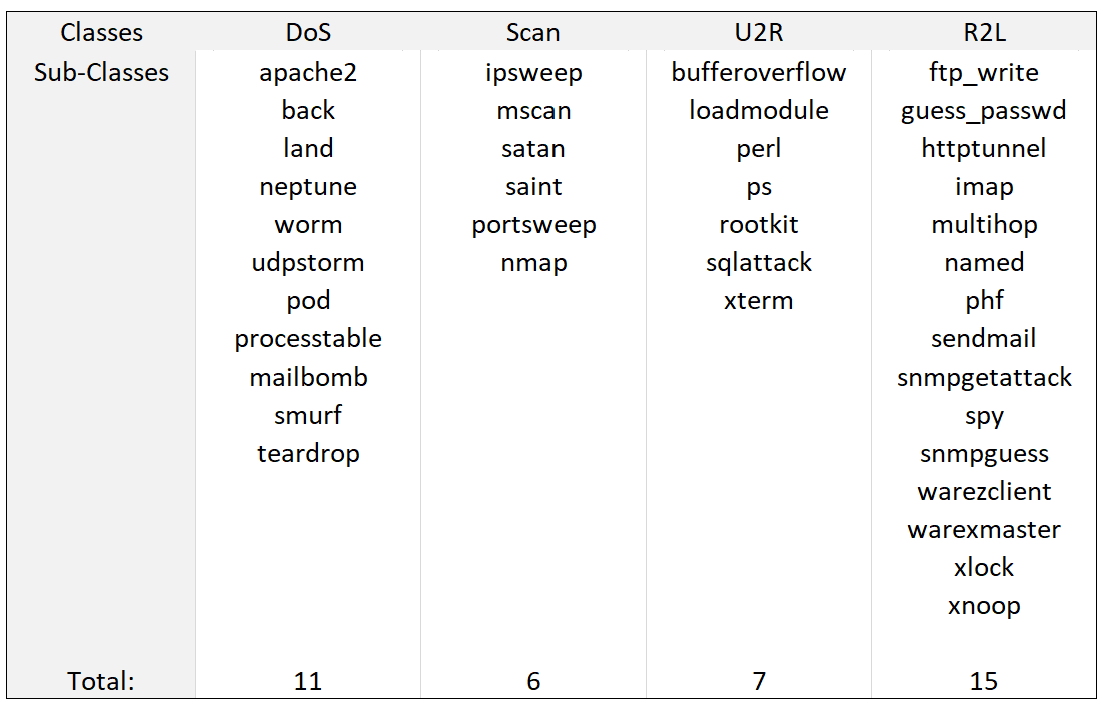
\includegraphics[totalheight=6cm]{figures/class-breakdown.png}
  \caption{List of all classes and sub-classes in the NSL-KDD set}
  \label{fig:class-breakdown}
  \centering
\end{figure}

The features include four main categories. The first is basic features, and include the protocol, port, service, and any flags. The basic features are found by inspecting the header of the incoming packet. Features 1-9 are basic features. The second category is payload. The payload features contain information about the payload of the packets as well as information about how the payload is split over multiple packets. Features 10-22 are payload features. The third category are short time-based features. Short time-based features are recorded over a 2-second window and contain information about how often attempts were made to connect to the host or how quickly packets came in. Features 23-31 are short time-based features. Finally, the last category are long time-based features. These features are recorded as requests over so many connections made to a host. Features 32-41 are long time-based features. The dataset is stored as a raw csv file containing both features and labels. For this reason, a small amount of pre-processing was required in order to format the data for the network. The following steps were taken in order to prepare the data:

\begin{itemize}
  \item data was shuffled and normalized
  \item labels and features were split into separate arrays
  \item text labels and features were enumerated
  \item categorical labels and features were one-hot encoded
\end{itemize}

\subsection{Model Design}

The goal of the model is to evaluate the network features contained in the NSL-KDD set and classify them as normal traffic or one of the four types of attacks. To achieve this goal, the model was built with two main sections: a deep encoder section and a dense network section. A layout of the network can be seen in figure~\ref{fig:network-structure}.

\begin{figure}[!htb]
  \centering
  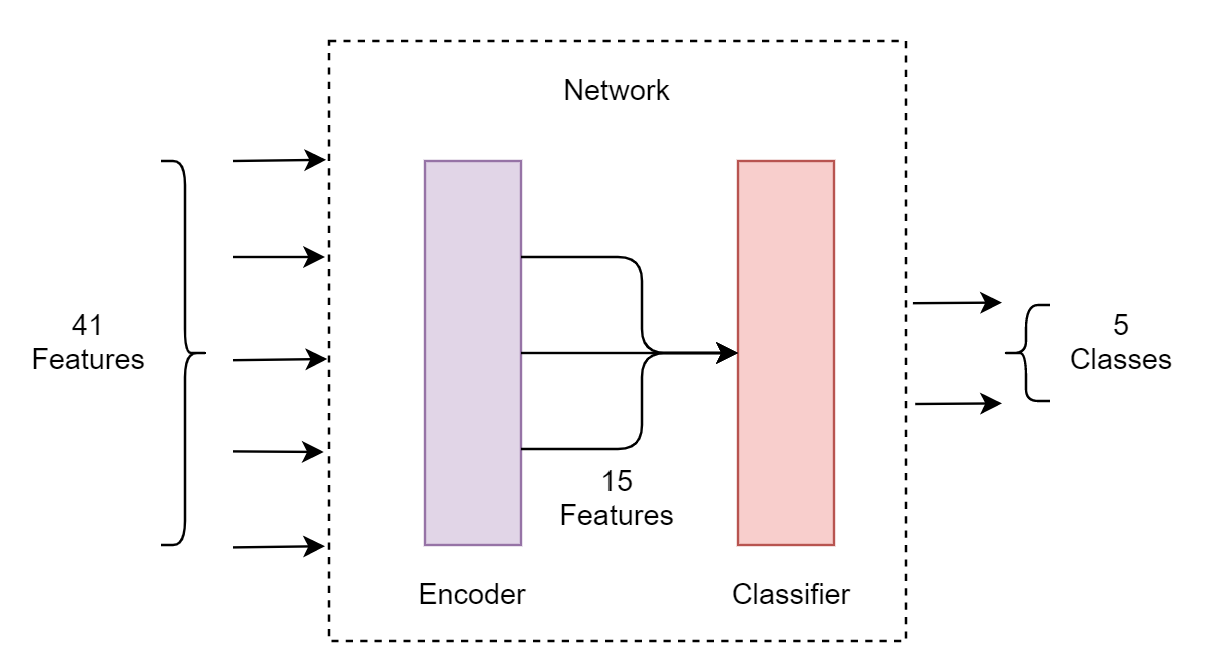
\includegraphics[totalheight=7cm]{figures/network-structure.png}
  \caption{Deep Network Structure}
  \label{fig:network-structure}
  \centering
\end{figure}

\subsubsection{Deep Encoder}

The motivation behind the encoder is to reduce the dimension of the data in order to allow the network to focus on important information. This is important due to how varied the classes are. Certain classes place much more importance on small sets of features than other classes do. For instance, the buffer overflow sub-class is very dependant on the payload, where the payload is usually not necessary to identify a DoS or Scan. By delivering compressed features to the classifier, the encoder allows the network to only focus on important information. The deep encoder section uses three layers to reduce the feature-set. An overview of the encoder section can be seen in figure~\ref{fig:encoder-structure}.

\begin{figure}[!htb]
  \centering
  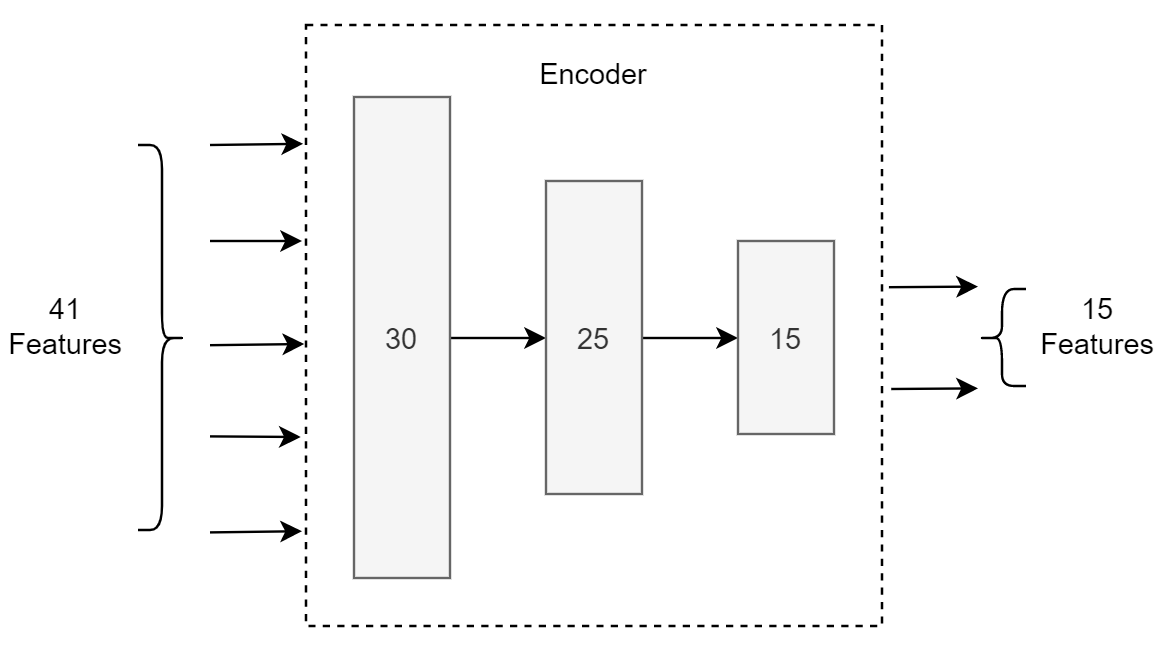
\includegraphics[totalheight=7cm]{figures/encoder-structure.png}
  \caption{Deep Encoder Structure for Dimensionality Reduction}
  \label{fig:encoder-structure}
  \centering
\end{figure}

\pagebreak
\subsubsection{Dense Network}

The dense network is designed to receive 15 features from the output of the encoder and learn to classify either normal operation or one of the four attack classes. The network is constructed using three dense layers with a rectified linear unit (ReLu) as the activation function. The network learns to map the reduced feature set to a five position vector before using a softmax layer to classify the datapoint. An overview of the classifier can be seen in figure~\ref{fig:dense-structure}.

\begin{figure}[!htb]
  \centering
  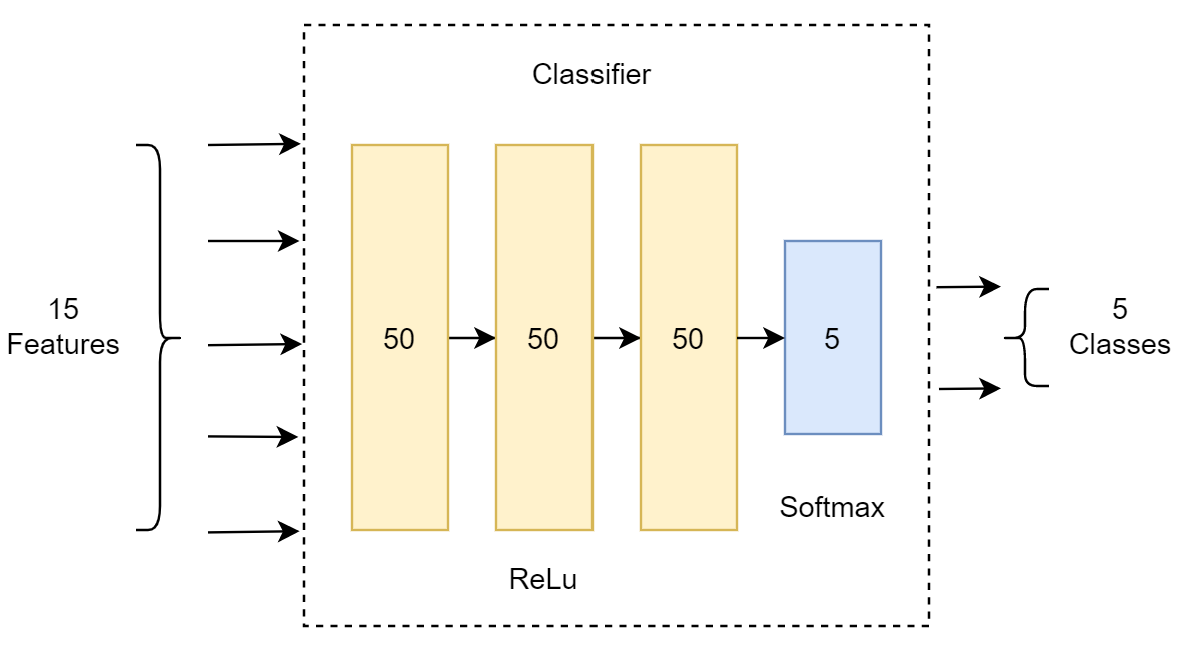
\includegraphics[totalheight=7cm]{figures/dense-structure.png}
  \caption{Dense Network Structure for Classification}
  \label{fig:dense-structure}
  \centering
\end{figure}

\subsection{Implementation}

The proposed model was implemented in in python 3 using keras and the tensorflow library. Other resources used include pandas for data storage and manipulation, numpy for data manipulation, matplotlib for viewing results, and sklearn for normalizing data and reporting statistics. The program uses pandas to load the dataset from a csv and formats the data into features and labels. The training and validation set are split at run time so that the model is validated on 20\% of the total dataset. The model is trained over 200 epochs and implements $\ell^2$ regularization with a rate of 0.1. In order to compensate for the low number of U2R records, the training set was over sampled by replicating U2R records. The number of U2R records were multiplied 10 times. Several results are obtained and stored while training the model. A custom callback has been written to store accuracy, loss, and training time at each epoch, which is plotted at the end of the model using the matplotlib library. In addition, the classification report function from the sklearn library is used to determine precision, recall, and the f1-score for each of the classes as the model runs.

\section{Evaluation}

The model was trained on the NSL-KDD dataset. Various metrics were evaluated for the model, including accuracy, precision, recall, and f1-score. The testing and training accuracy was recorded and plotted for every epoch of the model. The precision, recall, and f1-score for each class was recorded after the model was trained. The various metrics can be described as:

\begin{itemize}
  \item \textbf{Accuracy:} percentage of correctly classified records
  \[\text{\textit{Accuracy}} = \frac{\text{\textit{Correctly Classified Records}}}{\text{\textit{Total Records}}} \]
  \item \textbf{Precision:} percentage of correctly classified positive records
  \[\text{\textit{Precision}} = \frac{\text{\textit{Correctly Classified Positive Records}}}{\text{\textit{Total Classified Positive Records}}} \]
  \item \textbf{Recall:} percentage of correctly classified negative records
  \[\text{\textit{Recall}} = \frac{\text{\textit{Correctly Classified Negative Records}}}{\text{\textit{Total Classified Negative Records}}} \]
  \item \textbf{F1-Score:} accuracy taking into account precision and recall
  \[\text{\textit{F1-Score}} = 2 \times \frac{\text{\textit{Precision}} \times \text{\textit{Recall}}}{\text{\textit{Precision}} + \text{\textit{Recall}}} \]
\end{itemize}

It is important to note that while accuracy shows the models overall performance, it doesn't reflect the cost of false positives or false negatives made in the model. For this reason the F1-Score will be used as the true measure of how well the model performed. The model receives an overall accuracy of 98.5\% when trained over 200 epochs. The results of training the model can be seen in figure~\ref{fig:training-plot}. The results of the completed model can be seen in table~\ref{tab:model-results}.

\begin{figure}[!htb]
  \centering
  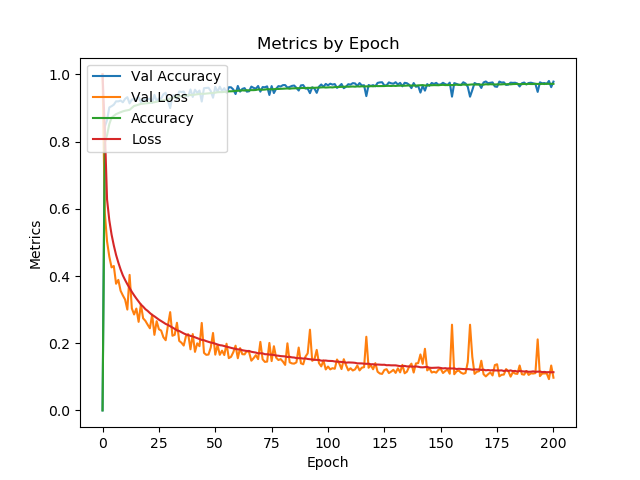
\includegraphics[totalheight=7cm]{figures/training-plot.png}
  \caption{Training and Testing Metrics by Epoch}
  \label{fig:training-plot}
  \centering
\end{figure}

\pagebreak

\begin{table}[!h]
\centering
\begin{tabular}{ |c|c|c|c|c|c|c| }
  \hline
  Class & Precision & Recall & F1-Score \\
  \hline
  Normal & 0.98 & 0.99 & 0.99 \\
  DoS    & 1.00 & 0.99 & 0.99 \\
  Scan   & 0.96 & 0.98 & 0.96 \\
  U2R   & 0.25 & 0.78 & 0.38 \\
  R2L    & 0.96 & 0.80 & 0.87 \\
  \hline
  Weighted Avg  & 0.98 & 0.98 & 0.98 \\
  \hline
\end{tabular}
\caption{Model Performance}
\label{tab:model-results}
\end{table}

The results show the precision, recall, and f1-score per class as well as the weighted average of the metrics. As can be seen in the table, the overall F1-Score is 98\%. The fact that the F1-Score is near the Accuracy shows that the model made very few false positive or negative classifications during the testing phase. The normal, DoS, and Scan classes achieve very high scores, the R2L class achieves reasonable scores, and the U2R class achieves poor scores. This is due to the number of records available for each class. The first three classes have a large number of records and the U2R class has a very small number of records. The U2R class achieved a poor precision and F1-Score, but a reasonable recall. The recall means that the model did not classify many records as U2R falsely, but the poor precision means that it also did not do well classifying U2R records correctly. The oversampling performed on the U2R records allow the model to learn the U2R class more easily, but it is not a sufficient alternative to real data. Overall, the model performed well and increasing the number of real records with the U2R label will help to increase the score of that class as well as the overall model. The proposed model was compared to the encoder-random forest model proposed by Shone et all. in~\cite{baseline1}. The results of that paper can be seen in table~\ref{tab:model-comparison}.

\begin{table}[!h]
\centering
\begin{tabular}{ |c|c|c|c|c|c|c| }
  \hline
  Class & Precision & Recall & F1-Score \\
  \hline
  Normal & 1.00 & 0.98 & 0.97 \\
  DoS    & 1.00 & 0.95 & 0.99 \\
  Scan   & 1.00 & 0.95 & 0.97 \\
  U2R    & 1.00 & 0.03 & 0.05 \\
  R2L    & 1.00 & 0.04 & 0.87 \\
  \hline
  Weighted Avg  & 1.00 & 0.85 & 0.87 \\
  \hline
\end{tabular}
\caption{Baseline Results~\cite{baseline1}}
\label{tab:model-comparison}
\end{table}

The method used to obtain these results was feature reduction using a stacked auto-encoder followed by classification using a random forest algorithm. As can be seen by the results, the random forest algorithm was more precise when making classifications but had poorer recall. In addition, the deep network performed better than the random forest algorithm when looking at the U2R and R2L classes, partially due to oversampling the U2R records. Comparing the f1-scores of both models, it is easy to see that the deep learning model, with a score of 98\%, outperforms the random forest model scoring at 87\%.

\section{Conclusion}

In conclusion, the proposed encoder-classifier model succeeded in classifying attacks with a high accuracy. The model reported an overall accuracy of 98\% and an average precision, recall, and f1-score of 98\%. These scores reflect how the model is able to correctly classify records without many false positive or negative classifications. The U2R classifier performed poorly in this model due to how few records there are in the NSL-KDD data set. This was slightly offset by oversampling the records in the training set to allow the model to see more records. While this improved the accuracy of the classifier when viewing U2R records, it is not a substitute for more independent records. The stacked encoder-classifier model overall performed well on the NSL-KDD dataset and will only improve as more data is obtained in the field of network intrusion detection.

\pagebreak

\bibliographystyle{IEEEtran}
\bibliography{references}

\end{document}
